\subsection{Гистограммы}
\begin{itemize}
	\item{Нормальное распределение}
	\begin{figure}[H]
		\begin{center}
			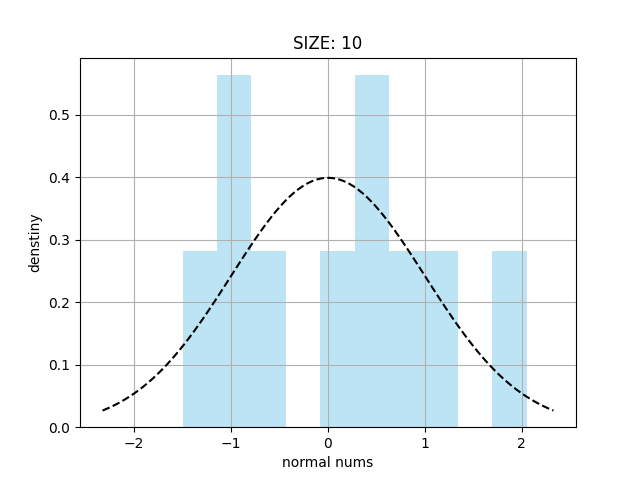
\includegraphics[scale=0.333]{resources/normal10.png}
			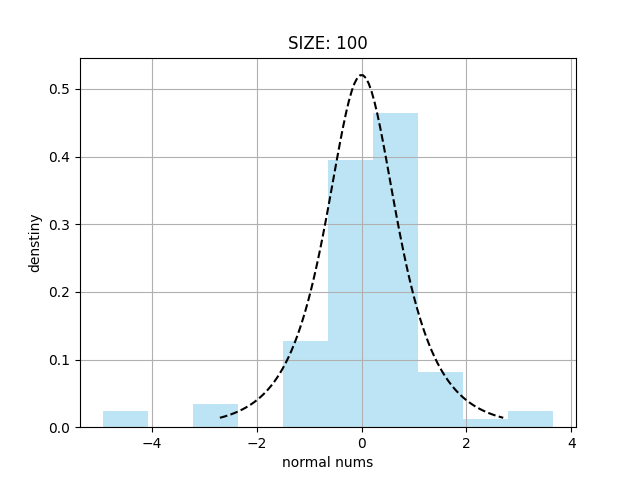
\includegraphics[scale=0.333]{resources/normal100.png}
			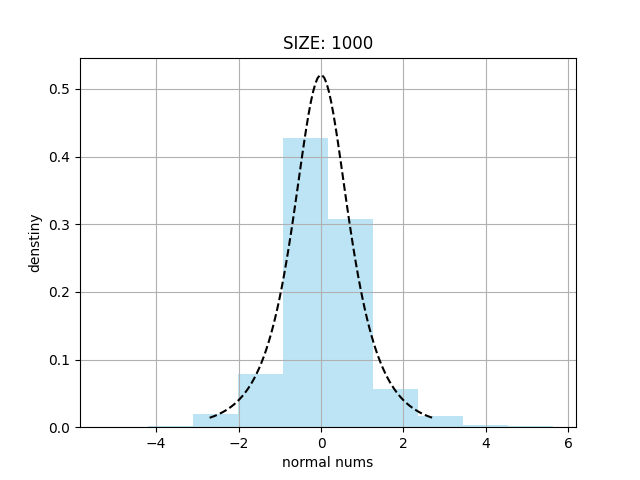
\includegraphics[scale=0.333]{resources/normal1000.png}
			\caption{Гистограмма и плотность вероятности для нормального распределения [N = 10, 100, 1000]} 
		\end{center}
	\end{figure}
	
	\item{Распределение Коши}
	\begin{figure}[H]
		\begin{center}
			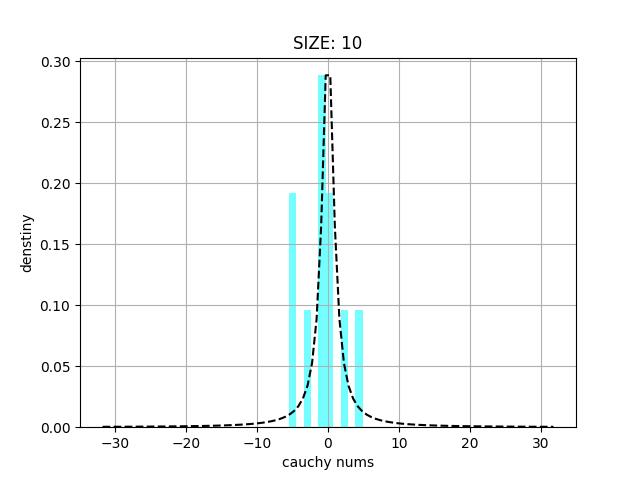
\includegraphics[scale=0.5]{resources/cauchy10.png}
			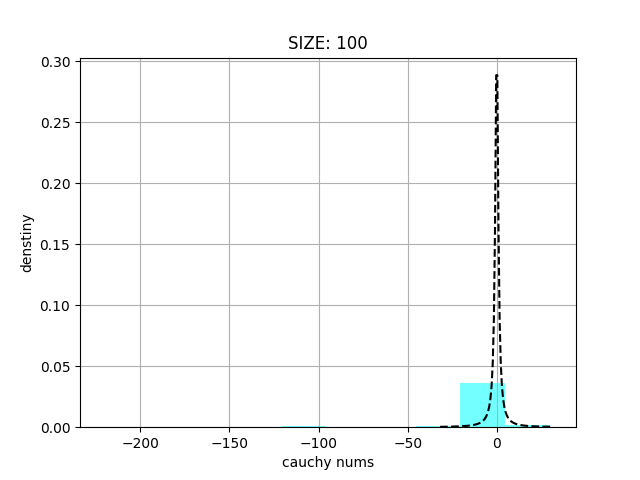
\includegraphics[scale=0.5]{resources/cauchy100.png}
			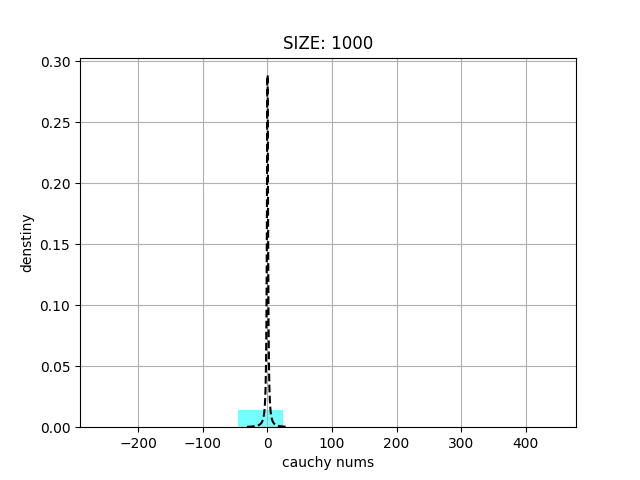
\includegraphics[scale=0.75]{resources/cauchy1000.png}
			\caption{Гистограмма и плотность вероятности для распределения Коши [N = 10, 100, 1000]}
		\end{center}
	\end{figure}
		
	\item{Распределение Пуассона}
	\begin{figure}[H]
		\begin{center}
			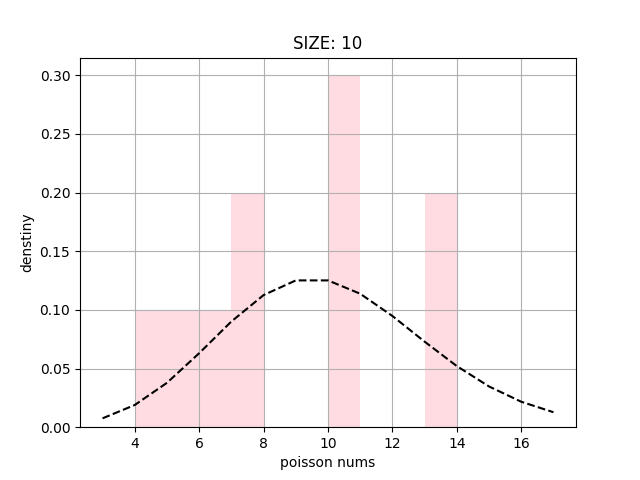
\includegraphics[scale=0.333]{resources/poisson10.png}
			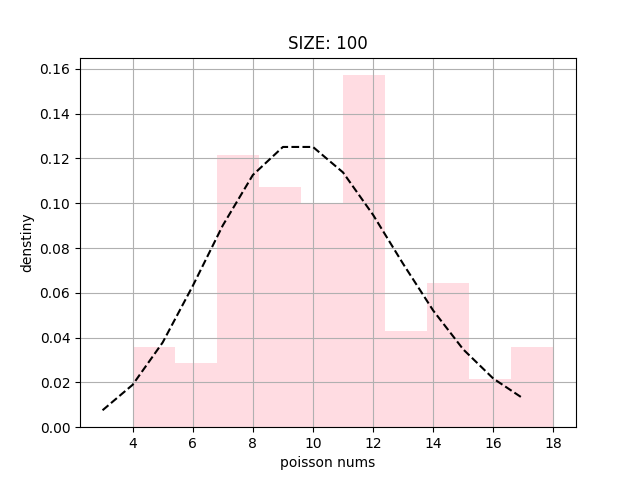
\includegraphics[scale=0.333]{resources/poisson100.png}
			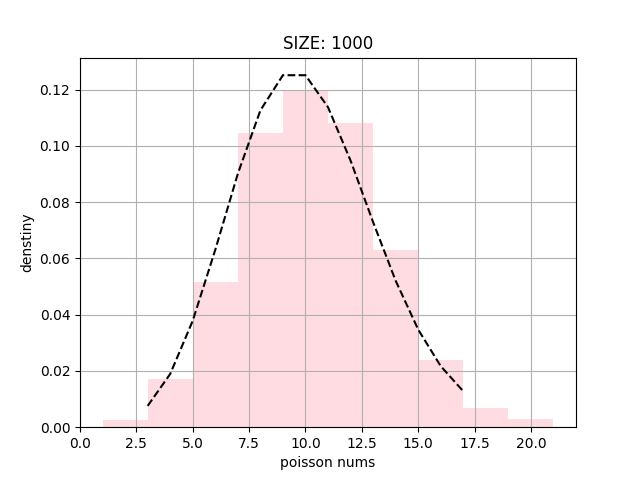
\includegraphics[scale=0.333]{resources/poisson1000.png}
			\caption{Гистограмма и плотность вероятности для распределения Пуассона [N = 10, 100, 1000]} 
		\end{center}
	\end{figure}
	
	\item{Равномерное распределение}
	\begin{figure}[H]
		\begin{center}
			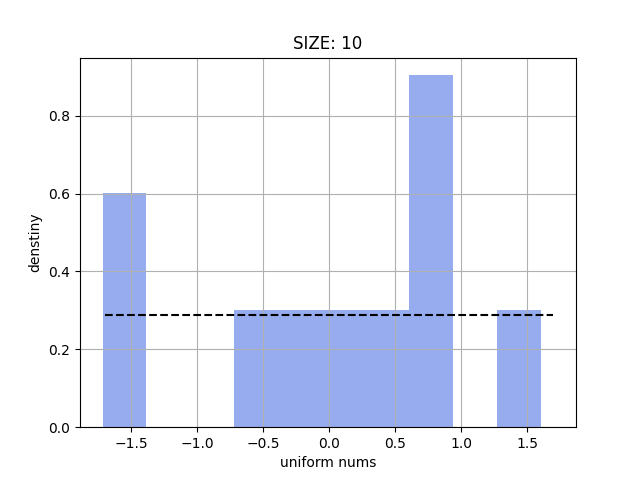
\includegraphics[scale=0.333]{resources/uniform10.png}
			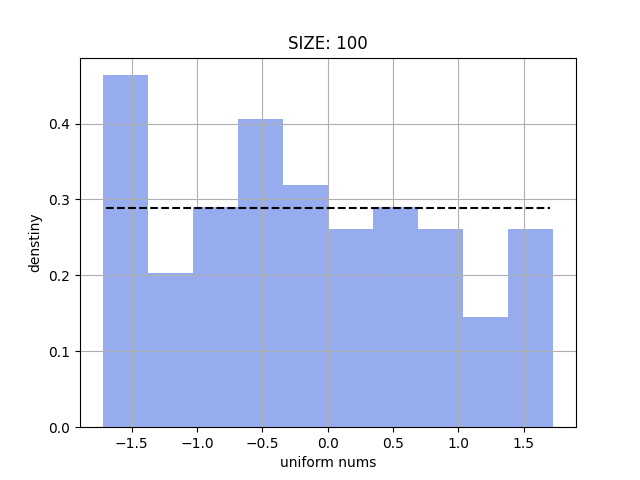
\includegraphics[scale=0.333]{resources/uniform100.png}
			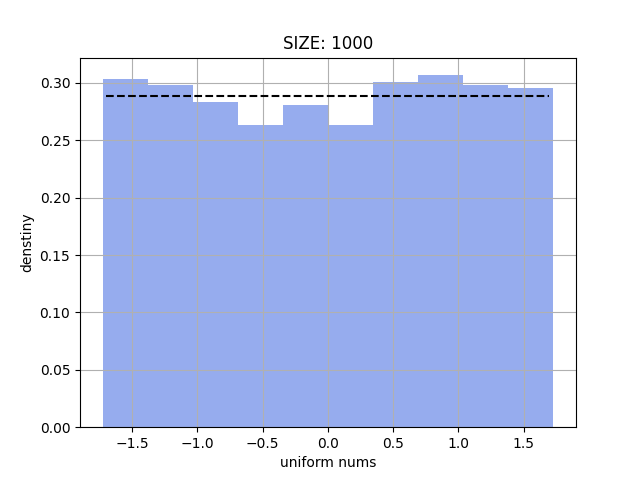
\includegraphics[scale=0.333]{resources/uniform1000.png}
			\caption{Гистограмма и плотность вероятности для равномерного распределения [N = 10, 100, 1000]} 
		\end{center}
	\end{figure}

\end{itemize}